%!TEX root = ../../report.tex

\begin{figure}[H]
	\newcommand{\figurewidth}{0.5\textwidth}
	\begin{subfigure}[b]{\figurewidth}
        \figureborder{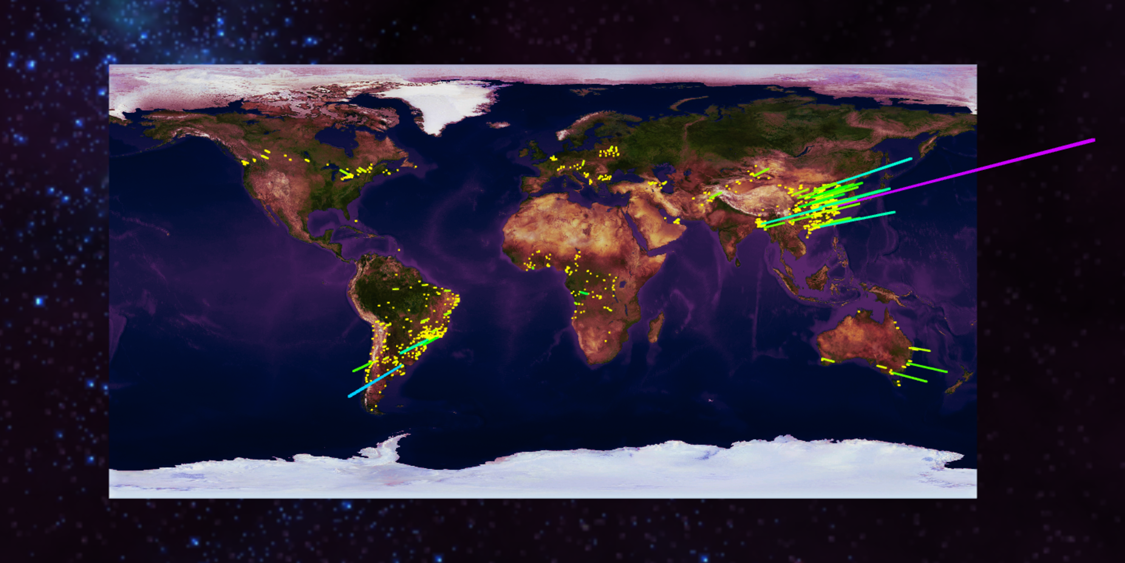
\includegraphics[width=\textwidth]{images/implementation/shaders/red}}
		\caption{Red midtone filter effect.}
		\label{fig:red_midtone}
	\end{subfigure}
	\begin{subfigure}[b]{\figurewidth}
		\figureborder{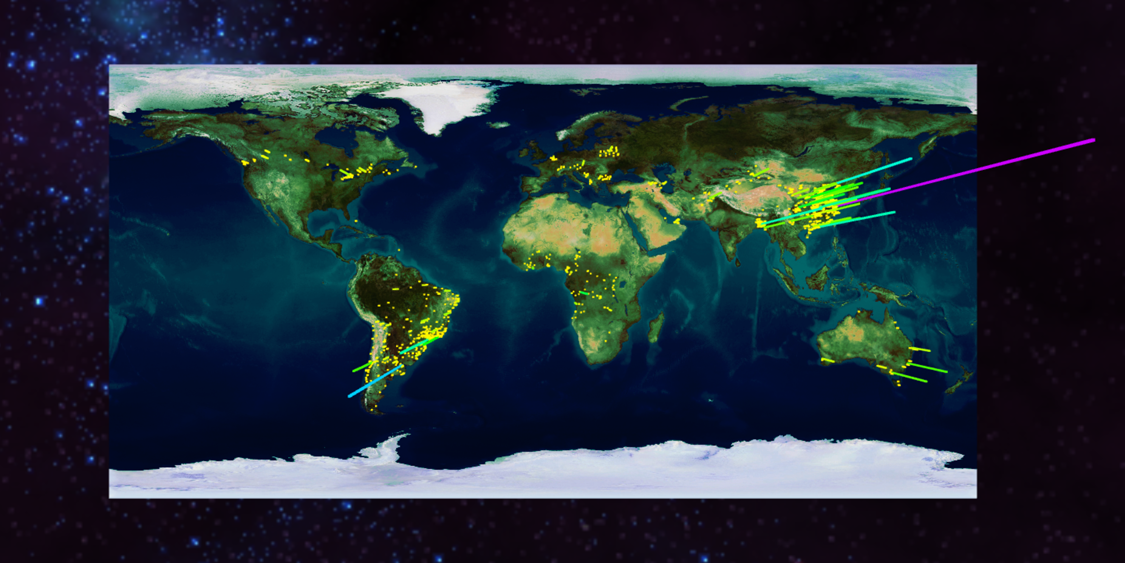
\includegraphics[width=\textwidth]{images/implementation/shaders/green}}
		\caption{Green midtone filter effect.}
		\label{fig:green_midtone}
	\end{subfigure}
	\begin{subfigure}[b]{\figurewidth}
		\figureborder{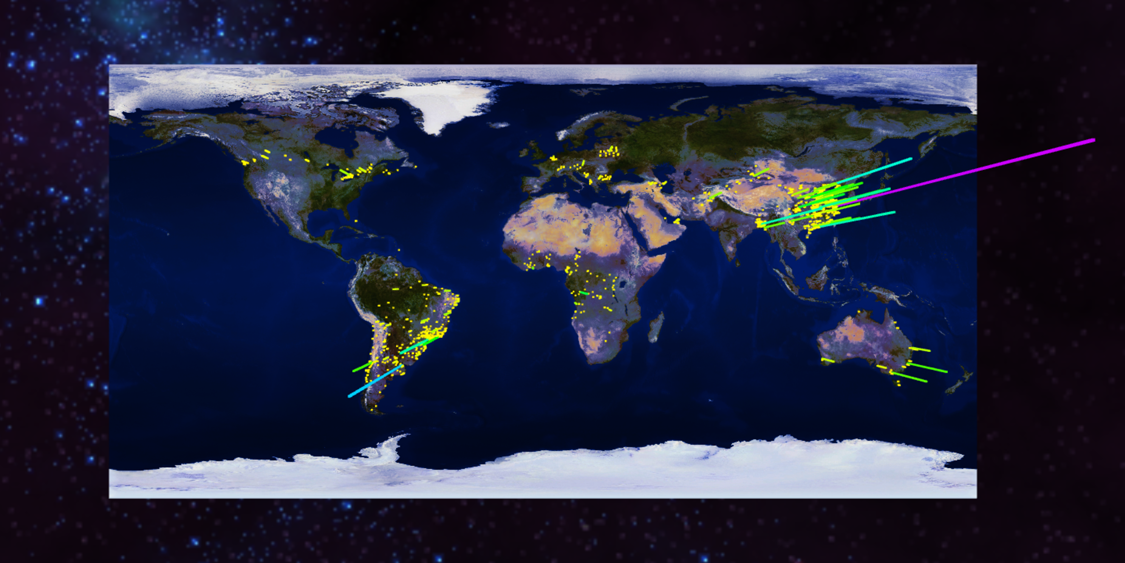
\includegraphics[width=\textwidth]{images/implementation/shaders/blue}}
		\caption{Blue midtone filter effect.}
		\label{fig:blue_midtone}
	\end{subfigure}
	\begin{subfigure}[b]{\figurewidth}
		\figureborder{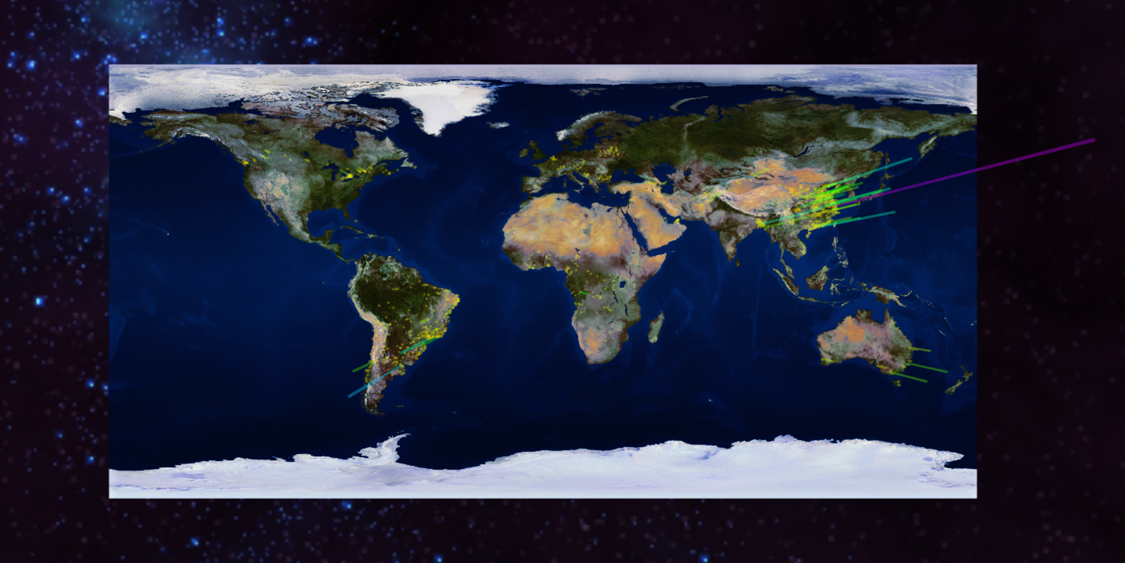
\includegraphics[width=\textwidth]{images/implementation/shaders/opacity}}
		\caption{Opacity filter effect.}
		\label{fig:opacity_filter}
	\end{subfigure}
	\begin{subfigure}[b]{\figurewidth}
		\figureborder{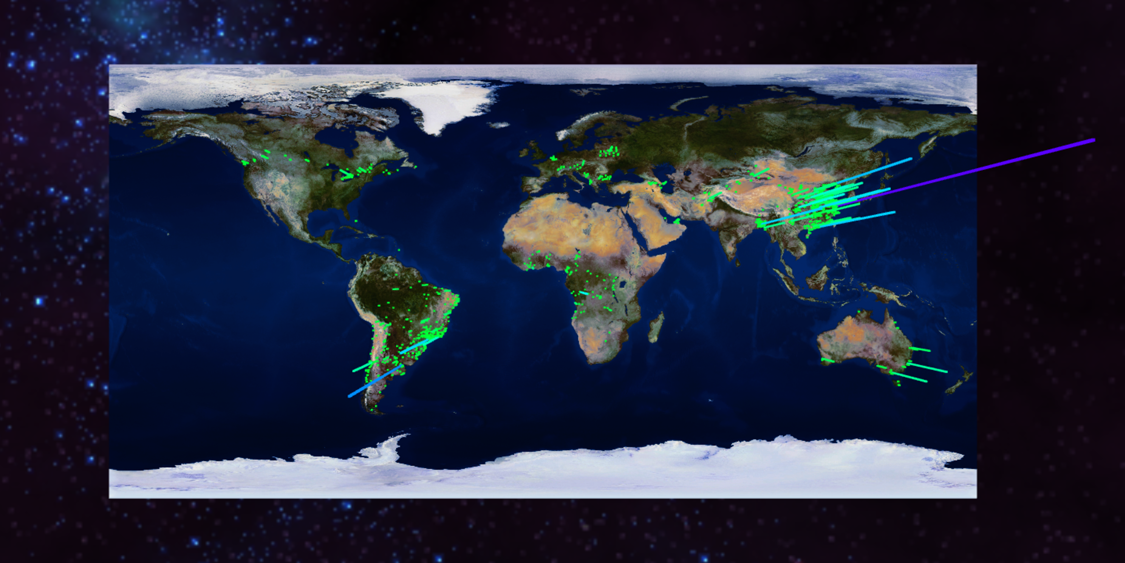
\includegraphics[width=\textwidth]{images/implementation/shaders/basic}}
		\caption{Alternate HSV colour range.}
		\label{fig:hsv_colour}
	\end{subfigure}
	\begin{subfigure}[b]{\figurewidth}
		\figureborder{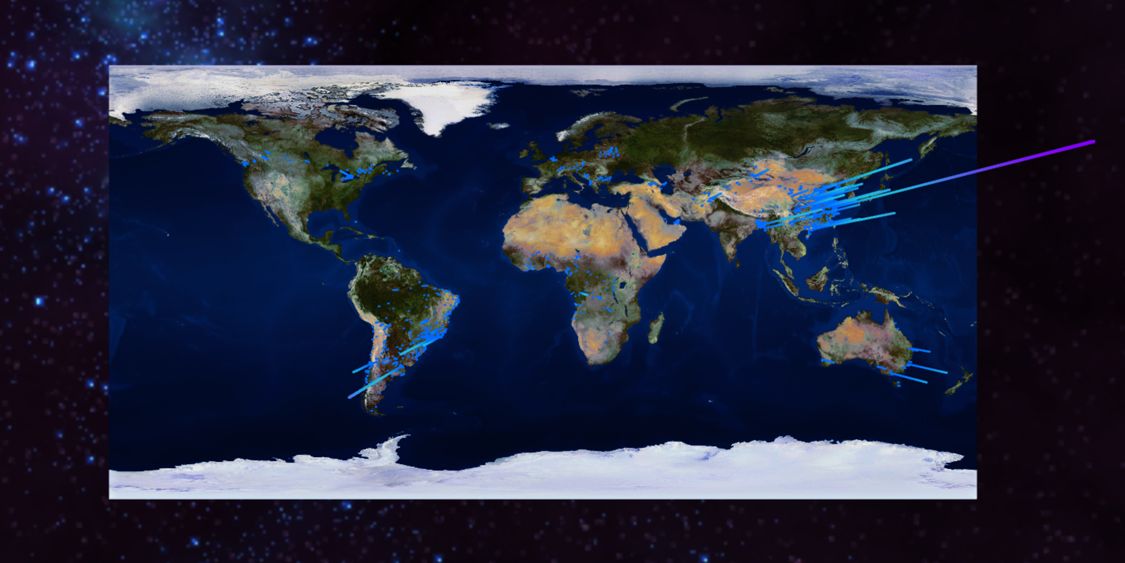
\includegraphics[width=\textwidth]{images/implementation/shaders/gradient}}
		\caption{Alternate gradient colour scheme.}
		\label{fig:gradient_colour}
	\end{subfigure}
	\caption[Shaders]{Available shader filter effects.}
	\label{fig:shaders}
\end{figure}
